\documentclass{article}
\usepackage{tikz}
\usepackage{pgfplots}
\usepackage{amsmath,amssymb}
\pgfplotsset{compat=newest}
\begin{document}
Exercise 1.2.6.\\
Find the standard equation of the circle passing through $(-2,1)$ and tangent to the line $3x-2y=6$ at the point $(4,3)$. Sketch.\\
\begin{enumerate}
    \item We will  solve $3x-2y=6$ for $y$ and graph it.
        \begin{align*}
            3x-2y&=6\\
            3x-6&=2y\\
            \frac{3}{2}x-3&=y
        \end{align*}
    \item We will plot the points $(-2,1)$ and $(4,3)$.
    \item We will graph the line perpendicular to $y=\frac{3}{2}x-3$ that passes through the point $(4,3)$.
    
        We know the slope is the negative reciprocal of $\frac{3}{2}$ and we have a point so we can solve for the y intercept by plugging these values into the $y=mx+b$ form.
        \begin{align*}
            y&=mx+b\\
            3&=-\frac{2}{3}(4)+b\\
            \frac{9}{3}&=-\frac{8}{3}+b\\
            b&=\frac{17}{3}\\
            y&=-\frac{2}{3}x+\frac{17}{3}
        \end{align*}
    \item the distance from the center of the circle to the point $(4,3)$ is the same as the distance to the point $(-2,1)$. So we will set the distance formulas equal to each other and solve for y. Then we will graph this and find its intercept with $y=\frac{3}{2}x-3$ which will be the center of the circle.
        \begin{align*}
            \sqrt{(x-(-2))^2+(y-1)^2}&=\sqrt{(x-4)^2+(y-3)^2}\\
            (x-(-2))^2+(y-1)^2&=(x-4)^2+(y-3)^2\\
            (x+2)^2+(y-1)^2&=(x-4)^2+(y-3)^2\\
            x^2+4x+4+y^2-2y+1&=x^2-8x+16+y^2-6y+9\\
            4x-2y+5&=-8x-6y+25\\
            4y&=-12x+20\\
            y&=-3x+5
        \end{align*}
    \item now we will solve for the intercept of $y=-3x+5$ and  $y=-\frac{2}{3}x+\frac{17}{3}$, and plot it.
        \begin{align*}
            -3x+5&=-\frac{2}{3}x+\frac{17}{3}\\
            -\frac{9}{3}x+\frac{15}{3}&=-\frac{2}{3}x+\frac{17}{3}\\
            \frac{7}{3}&=-\frac{2}{3}\\
            x&=-\frac{2}{7}\\
            y&=-3\left(-\frac{2}{7}\right)+\frac{35}{7}\\
            y&=\frac{41}{7}
        \end{align*}
    \item Now we will solve for the radius of the circle.
        \begin{align*}
            \sqrt{(\Delta x)^2+(\Delta y)^2}&=\sqrt{\left(4-\left(-\frac{2}{7}\right)\right)^2+\left(3-\frac{41}{7}\right)^2}\\
            &=\sqrt{\left(\frac{30}{7}\right)^2+\left(\frac{400}{49}\right)^2}\\
            &=\sqrt{\frac{1300}{49}}\\
            &=\frac{10\sqrt{13}}{7}
        \end{align*}
    \item now we express the formula for the circle, and draw it.

    \[\left(x+\frac{2}{7}\right)^2+\left(y-\frac{41}{7}\right)^2=\frac{1300}{49}\]
\end{enumerate}

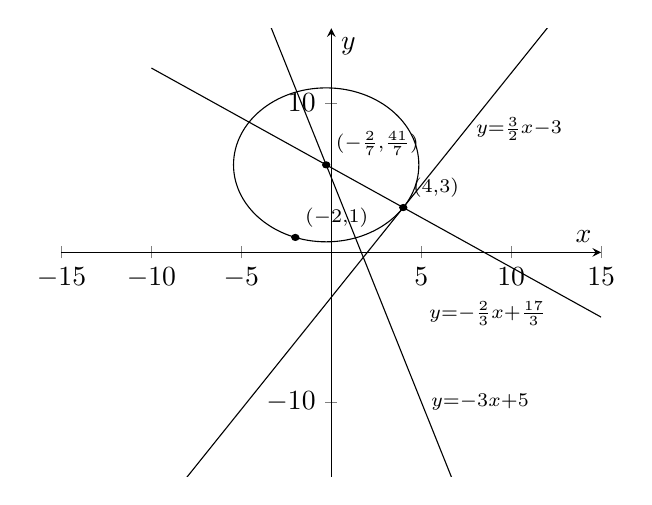
\begin{tikzpicture}
\begin{axis}[
axis lines=middle,
ylabel={$y$},
xlabel={$x$},
ymax=15, ymin=-15,
xmax=15, xmin=-15,
domain=-10:15
]
\addplot[]{(3/2)*x-3} node[pos=.7,right]{$\scriptstyle y=\frac{3}{2}x-3$};
\draw[fill] (-2,1) circle [radius=0.2] node[above right] {$\scriptstyle(-2,1)$};
\draw[fill] (4,3) circle [radius=0.2] node[above right] at (4,3) {$\scriptstyle(4,3)$};
\addplot[]{-(2/3)*x+(17/3)} node[pos=.9,below left]{$\scriptstyle y=-\frac{2}{3}x+\frac{17}{3}$};
\addplot[]{-3*x+5} node[pos=.6,right]{$\scriptstyle y=-3x+5$};
\draw[fill] (-2/7,41/7) circle [radius=0.2] node[above right] {$\scriptstyle(-\frac{2}{7},\frac{41}{7})$};
\draw (-2/7,41/7) circle [radius=10*sqrt(13)/7];
\end{axis}
\end{tikzpicture}
\end{document}